\section{Groupes et formulaires}\label{sec:groupes-et-formulaires}

Le cœur du projet est un éditeur de formulaires.
Cet éditeur permet de fabriquer un schéma, qui est ensuite utilisé pour générer l'interface de saisie et pour valider les saisies.

Pour cela, on définit plusieurs termes :
\begin{itemize}
	\item Champ : une donnée demandée à l'utilisateur, qui peut être simple (du texte, un numéro de téléphone…) ou posséder des sous-champs (choisir entre plusieurs options).
	Ils sont représentés par des structures récursives, dont la racine dicte des contraintes spécifiques.
	\item Formulaire : un groupement de champs ayant un nom, pouvait être accessible par les administrés,
	\item Groupe : un groupement de champs ayant un nom, représentant un morceau d'un formulaire, pouvant être réutilisé au sein de plusieurs formulaires (similaire à un patron de formulaire).
\end{itemize}

\paragraph{Familles de champs}
Il existe cinq familles de champs :
\begin{itemize}
	\item Les champs d'affichage de texte, qui permettent d'afficher un simple texte à l'utilisateur,
	\item Les champs simples, qui n'ont pas de sous-champs et représentent les champs traditionnels (addresse mail, numéro de téléphone…),
	\item Les champs composés, qui représentent un ensemble de sous-champs que l'utilisateur doit remplir,
	\item Les champs unions, qui représentent un ensemble de sous-champs dont l'utilisateur ne remplit qu'un,
	\item Les champs listes, qui n'ont pas de sous-champs et représentent un champ qui peut être rempli plusieurs fois.
\end{itemize}
Ces différentes familles sont implémentées de manière très différente les unes des autres, mais aussi d'une racine à une autre.

\subparagraph{Champs simple et affichage de texte}
Il existe de nombreux types de champs simples, qui sont implémentés par la classe scéllée \lstinline{SimpleField}.
Parmi ces implémentations, on retrouve les cases à cocher (\lstinline{SimpleField.Boolean}), les addresses mail (\lstinline{SimpleField.Email}), les fichiers à téléverser (\lstinline{SimpleField.Upload}), etc.

Pour pouvoir afficher un texte simple à l'utilisateur n'importe où dans le formulaire (mentions légales, explications sur les décisions, aide…), il existe un cas particulier du champ simple, le champ «~texte non-modifiable~» (\lstinline{SimpleField.Message}).
Contrairement à tous les autres champs, celui-ci ne peut pas être rempli par l'utilisateur.
Pour éviter d'avoir à ajouter une interface de plus à la hiérarchie, il est implémenté comme un cas particulier d'un champ simple.

Les champs simples peuvent avoir des métadonnées en plus, selon le type.
Par exemple, on peut préciser la longueur maximale d'un texte, les formats autorisés pour une pièce jointe, etc.

\subparagraph{Unions}
Les unions (appelées «~choix~» dans l'interface web) permettent de créer un formulaire où l'utilisateur a le choix entre plusieurs champs.
Pour cela, les unions possèdent une liste de sous-champs, dont un seul peut être rempli par l'utilisateur.

Cette manière de faire est très puissante, mais n'est pas intuitive pour les administrateurs.
Puisqu'un choix implique une réponse unique, placer un champ simple «~bouton à cocher~» dans un choix implique l'affichage de \emph{deux} boutons, celui du choix correspondant à choisir cette option et le bouton lui-même.
Dans la majorité des cas, au lieu d'utiliser des boutons à cocher, on souhaite utiliser du texte non-modifiable :
\begin{lstlisting}[label={lst:lstlisting}]
Choix : « Genre »
	Texte non-modifiable : « Homme »
	Texte non-modifiable : « Femme »
	Texte modifiable : « Autre »
\end{lstlisting}

\subparagraph{Champs composés}
Les champs composés sont similaires aux unions, mais affichent tous les champs à l'utilisateur.

Contrairement aux unions, les champs composés ne peuvent se trouver qu'à la racine d'un arbre de champs --- et la racine d'un arbre de champs est obligatoirement un champ composé.
On ne peut donc pas créer de champs composés directement à l'intérieur dans un formulaire.

Au lieu de créer un champ composé dans un formulaire, on crée un groupe de champs, qui pourra ensuite être utilisé dans plusieurs formulaires.
Pour insérer un groupe de champs dans un formulaire, on utilise un champ «~référence~», qui permet de réutiliser ce groupe.
Ces champs référence permettent aussi d'utiliser un groupe à l'intérieur d'un autre groupe, ou même à l'intérieur de lui-même.

Les champs référence permettent de modifier certains attributs des champs référencés, par exemple l'arité.
Toutes les modifications doivent cependant être compatibles\footnote{Cette restriction provient du but original d'utiliser les groupes pour effectuer des recherches à travers tous les formulaires dont un groupe fait partie. Pour des raisons de temps, cela n'a pas été implémenté, mais la restriction est gardée en place pour le permettre dans le futur.} avec les champs originaux, il est donc recommandé de créer des groupes n'étant pas trop restrictifs.

\subparagraph{Listes}
Au lieu de représenter les listes par un type spécifique, elles sont représentées par une classe \lstinline{Arity}.
L'arité d'un champ est définie comme le nombre de réponses autorisées pour ce champ (nombre de réponses autorisées au minimum et au maximum).

Tous les champs possèdent une arité, un champ n'étant pas une liste a donc une arité maximale de 1 ou moins.
Il n'est donc pas nécessaire d'ajouter un type «~Liste~».

\uparagraph
Ces différentes familles de champs sont représentées par des interfaces, qui sont détaillées dans la figure \cnpref{fig:uml-fields}.

\begin{figure}[tp]
	\caption{Diagrammes UML de classes du fichier \lstinline{Field.kt}}
	\label{fig:uml-fields}
	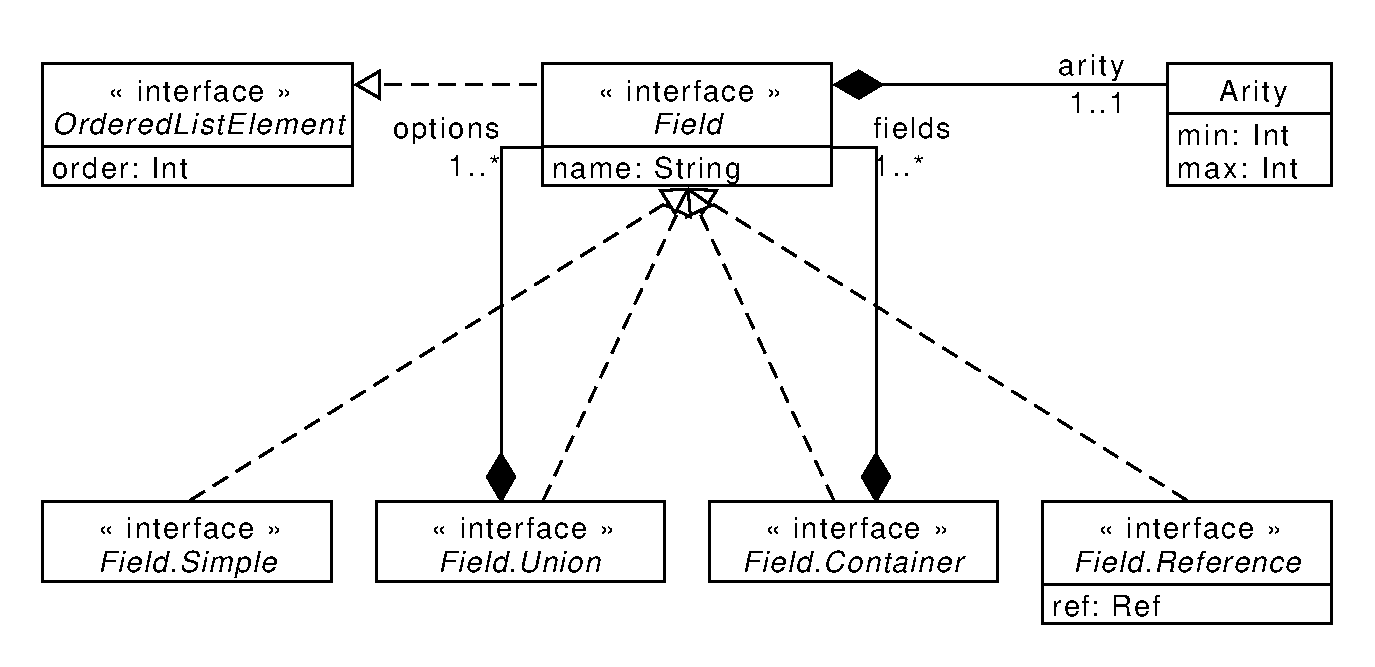
\includegraphics[width=\textwidth]{reports-forms-fields}
\end{figure}

\paragraph{Contextes}
Comme dit précédemment, les champs forment des arbres récursifs dont la racine dicte certaines informations.
Il existe trois racines différentes :
\begin{itemize}
	\item Les groupes,
	\item Les champs concrets d'un formulaire,
	\item Les champs référence d'un formulaire.
\end{itemize}

\subparagraph{Champs dans un groupe}
Dans un groupe, on retrouve des champs simples (\lstinline{DataField.Simple}), des unions (\lstinline{DataField.Union}), et des références vers d'autres groupes (\lstinline{DataField.Composite}).

Contrairement aux références dans les formulaires, il n'est pas possible de modifier les sous-champs.
Les références peuvent référencer d'autres groupes ou le groupe actuel lui-même (groupe récursif).
Les références vers d'autres groupes sont obligatoirement facultatives (sinon, il serait possible de créer un cycle récursif obligatoire, qui serait infini).
Quand un groupe est ajouté à un formulaire, il est possible de rendre plus stricte son arité (rendre le groupe facultatif obligatoire), donc cela n'a pas d'impact sur les possibilités de création de formulaire.

\subparagraph{Champs dans un formulaire}
Les formulaires sont séparés en deux niveaux, dont le code commun est placé dans l'interface \lstinline{FormField} :
\begin{itemize}
	\item Le niveau supérieur (proche de la racine), dans lequel les champs sont nouveaux,
	\item Le niveau inférieur (séparé de la racine par un nœud de type \lstinline{ShallowFormField.Composite}), dans lequel les champs sont des références à un groupe.
\end{itemize}

Le niveau supérieur (\lstinline{ShallowFormField}) peut contenir des champs simples (\lstinline{ShallowFormField.Simple}), des unions (\lstinline{ShallowFormField.Union}) et des références vers des groupes (\lstinline{ShallowFormField.Composite}).
Dans un formulaire, il est possible de modifier certains aspects des champs provenant des groupes (arité, métadonnées d'un champ simple, etc).
Les descendants d'une référence vers un groupe ne permettent que de modifier les champs autorisés, et héritent des autres (héritage par composition).
On retrouve donc une deuxième implémentation de chaque type qui ne stocke que les données qui peuvent être modifiées, pour les champs simples (\lstinline{DeepFormField.Simple}), pour les unions (\lstinline{DeepFormField.Union}) et pour les références vers d'autres groupes (\lstinline{DeepFormField.Composite}).
